% =============================================================
%  Project slides — Counterfactual Reasoning for Bias Mitigation
%  Compile with pdfLaTeX. Metropolis theme (Overleaf-ready).
% =============================================================
\documentclass[aspectratio=169,10pt]{beamer}

% --- Theme -------------------------------------------------------------
\usetheme{metropolis}
\usepackage[utf8]{inputenc}
\usepackage[T1]{fontenc}
\usepackage{graphicx}
\usepackage{booktabs}
\usepackage{tabularx}
\usepackage{amsmath,amssymb}
\usepackage{xcolor}
\usepackage{tikz}
\usetikzlibrary{arrows.meta, positioning, calc}

% --- Colour palette (matches report) -----------------------------------
\definecolor{goodgreen}{RGB}{39,174,96}
\definecolor{badred}{RGB}{192,57,43}
\definecolor{cfblue}{RGB}{41,128,185}
\definecolor{accent}{RGB}{243,156,18}
\setbeamercolor{progress bar}{fg=accent}
\setbeamercolor{frametitle}{bg=black!80}

\newcommand{\good}[1]{\textcolor{goodgreen}{\textbf{#1}}}
\newcommand{\bad}[1]{\textcolor{badred}{\textbf{#1}}}
\newcommand{\cf}[1]{\textcolor{cfblue}{\textbf{#1}}}
\newcommand{\acc}[1]{\textcolor{accent}{\textbf{#1}}}

% --- Title material ----------------------------------------------------
\title{Counterfactual Reasoning for Popularity-Bias Mitigation}
\subtitle{An LLM-Augmented Causal Framework on MovieLens-1M}
\date{April 2026}
\author{Project Presentation}
\institute{MovieLens-1M \,|\, 6{,}040 users $\times$ 3{,}883 movies $\times$ 1M ratings}

\begin{document}

% =================================================================
\begin{frame}
  \titlepage
  \vspace{-0.5em}
  \begin{center}
  \large
    \good{Zero-shot LLM MAB: $0.62$} \quad$\longrightarrow$\quad
    \good{Our framework: $0.026$}\\[2pt]
    \small (a $\sim$\textbf{96\%} reduction without losing accuracy)
  \end{center}
\end{frame}

% =================================================================
\begin{frame}{The Problem: Popularity Bias in Recommender Systems}
  \begin{columns}[T,onlytextwidth]
    \begin{column}{0.55\textwidth}
      \textbf{Popularity bias}
      \begin{itemize}
        \item Popular items get over-recommended, niche items under-recommended.
        \item Creates an exposure feedback loop — hurts creators and users with
              atypical preferences.
        \item \cf{Even good CF models have it:} SVD has $+0.19$ bias on niche,
              $+0.08$ on blockbusters.
      \end{itemize}
      \vspace{0.4em}
      \textbf{How we measure it}
      \begin{itemize}
        \item \emph{Mean Absolute per-bucket Bias (MAB):}
              $\tfrac{1}{5}\sum_b |\bar{\hat r}_b - \bar r_b|$
              over 5 popularity quintiles.
        \item Lower MAB $\Rightarrow$ fairer predictions across popularity.
      \end{itemize}
    \end{column}
    \begin{column}{0.43\textwidth}
      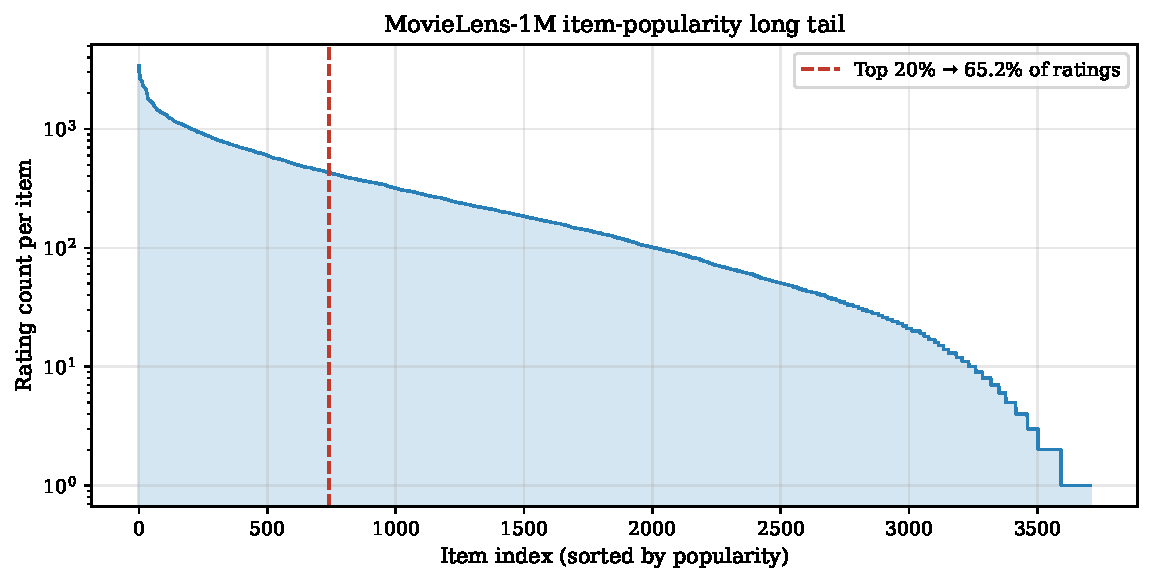
\includegraphics[width=\linewidth]{figures/longtail.pdf}
      \begin{center}\scriptsize
        Top 20\% of items account for most ratings.\\
        Classical long tail.
      \end{center}
    \end{column}
  \end{columns}
\end{frame}

% =================================================================
\begin{frame}{LLMs Make it Worse}
  \begin{columns}[T,onlytextwidth]
    \begin{column}{0.52\textwidth}
      \textbf{Why a zero-shot LLM is biased}
      \begin{itemize}
        \item Pre-training corpus over-represents mainstream films.
        \item Confident predictions skewed toward cultural conformity.
        \item Hallucinates post-hoc rationales defending popular picks.
      \end{itemize}
      \vspace{0.4em}
      \textbf{Measured on MovieLens-1M (Qwen2.5-14B)}
      \begin{itemize}
        \item Overall bias: \bad{$+0.62$} stars
        \item Blockbuster bias: \bad{$+0.43$}
        \item $\sim$5$\times$ worse than SVD on the same bucket ($+0.43$ vs $+0.08$).
      \end{itemize}
    \end{column}
    \begin{column}{0.47\textwidth}
      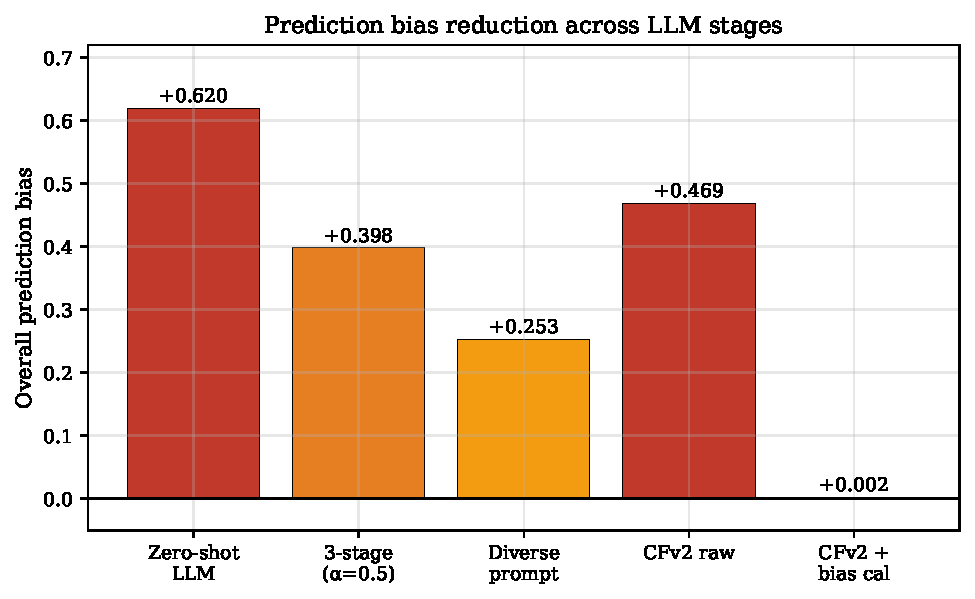
\includegraphics[width=\linewidth]{figures/bias_reduction.pdf}
      \begin{center}\scriptsize
        Bias trajectory across LLM stages.
      \end{center}
    \end{column}
  \end{columns}
\end{frame}

% =================================================================
\begin{frame}{Our Idea: Causal Reasoning to Separate $M$ from $P$}
  \centering
  Rating $r$ is caused by a user--item \cf{semantic match $M$} \emph{and}
  confounded by the item's \bad{popularity $P$}.

  \vspace{0.6em}
  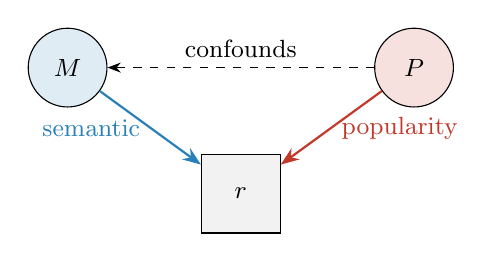
\begin{tikzpicture}[>=Stealth, node distance=1.4cm, font=\small]
    \node[draw, circle, fill=cfblue!15, minimum size=1.0cm] (M) at (-2.2,0.7) {$M$};
    \node[draw, circle, fill=badred!15, minimum size=1.0cm] (P) at ( 2.2,0.7) {$P$};
    \node[draw, rectangle, fill=black!5, minimum size=1.0cm] (R) at ( 0.0,-0.9) {$r$};
    \draw[->, thick, cfblue] (M) -- (R) node[midway,left] {semantic};
    \draw[->, thick, badred] (P) -- (R) node[midway,right] {popularity};
    \draw[->, dashed]        (P) -- (M) node[midway,above] {confounds};
  \end{tikzpicture}

  \vspace{0.6em}
  \textbf{Counterfactual intervention: $do(P \!\leftarrow\! \text{uniform})$}
  \vspace{0.3em}
  \begin{itemize}
    \item Force the LLM to predict $r$ as if popularity were equalised.
    \item Sever the $P \rightarrow r$ arrow via propensity re-weighting.
    \item Leave only the \cf{semantic match $M$} as the driver of the prediction.
  \end{itemize}
\end{frame}

% =================================================================
\begin{frame}{Method: 3-Stage Counterfactual Pipeline}
  \centering
  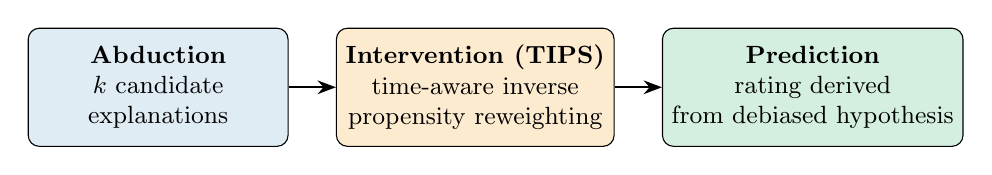
\begin{tikzpicture}[>=Stealth, node distance=0.6cm, font=\small]
    \node[draw, rounded corners, fill=cfblue!15, minimum width=3.3cm,
          minimum height=1.5cm, align=center] (A)
          {\textbf{Abduction}\\ $k$ candidate\\ explanations};
    \node[draw, rounded corners, fill=accent!20, right=of A,
          minimum width=3.3cm, minimum height=1.5cm, align=center] (I)
          {\textbf{Intervention (TIPS)}\\ time-aware inverse\\ propensity reweighting};
    \node[draw, rounded corners, fill=goodgreen!20, right=of I,
          minimum width=3.3cm, minimum height=1.5cm, align=center] (P)
          {\textbf{Prediction}\\ rating derived\\ from debiased hypothesis};
    \draw[->, thick] (A) -- (I);
    \draw[->, thick] (I) -- (P);
  \end{tikzpicture}
  \vspace{0.6em}
  \begin{itemize}\itemsep2pt
    \item \textbf{Abduction.} Inference-to-best-explanation: LLM generates $k{=}5$
          candidate textual reasons why the user might rate this item.
    \item \textbf{Intervention.} TIPS re-weights candidates by popularity-reliance:
          \[ S_k = (1-\alpha)\,\text{plausibility}_k \;-\; \alpha\,\text{pop\_reliance}_k \cdot \tfrac{\text{TIPS}_i^{(t)}}{\max_j \text{TIPS}_j^{(t)}}\]
    \item \textbf{Prediction.} Emit rating strictly from the selected debiased explanation.
  \end{itemize}
\end{frame}

% =================================================================
\begin{frame}{Baseline Selection: Bias Exists Even in Classical CF}
  \begin{columns}[T,onlytextwidth]
    \begin{column}{0.46\textwidth}
      \textbf{We measured bias on the notebook baselines:}
      \begin{itemize}\itemsep0pt
        \item \textbf{ARP} — avg.\ recommendation popularity
        \item \textbf{Coverage} — \% of catalogue ever recommended
      \end{itemize}
      \vspace{0.3em}
      \scriptsize
      \begin{tabular}{lccc}
        \toprule
        Model & RMSE & ARP $\downarrow$ & Cov. $\uparrow$ \\ \midrule
        Global Mean     & 1.147 & 2801 & \bad{0.3\%} \\
        Bias Model      & 0.922 & 1038 & 1.7\%  \\
        User-User KNN   & 0.922 & 1788 & 19.5\% \\
        Item-Item KNN   & 1.013 & \good{636}  & \good{88.1\%} \\
        \good{SVD (k=50)} & \good{0.893} & 1101 & 18.9\% \\
        \bottomrule
      \end{tabular}
    \end{column}
    \begin{column}{0.52\textwidth}
      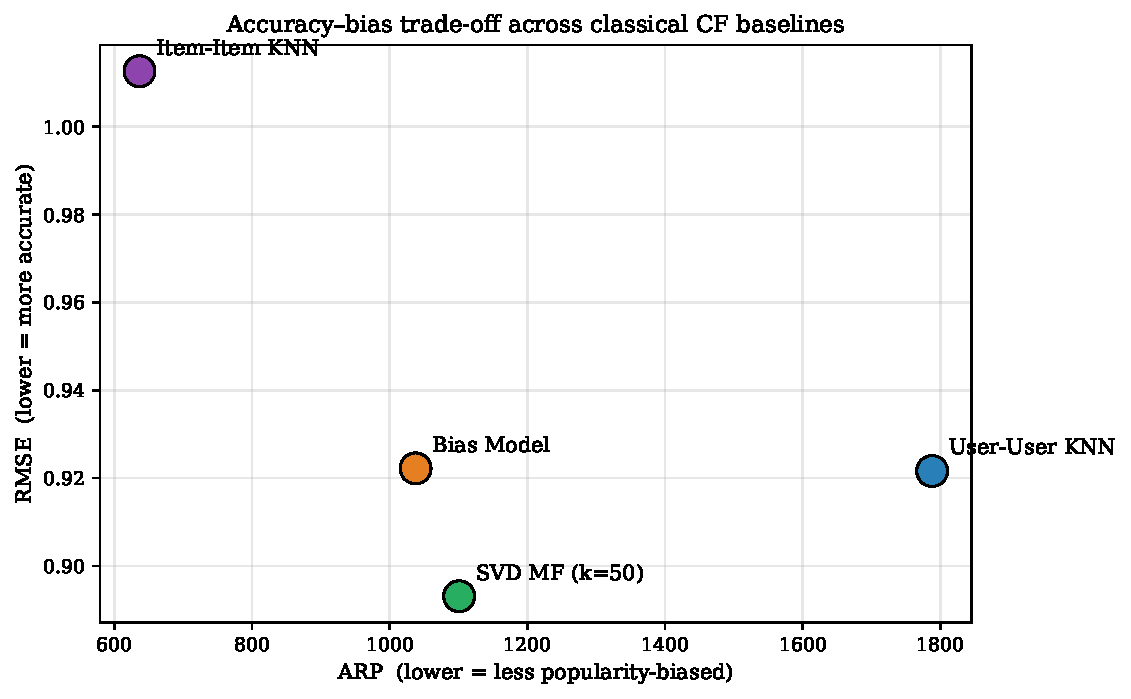
\includegraphics[width=\linewidth]{figures/accuracy_bias_tradeoff.pdf}
      \begin{center}\scriptsize
        Accuracy–bias trade-off across classical CF.
      \end{center}
    \end{column}
  \end{columns}
  \vspace{0.3em}
  \footnotesize
  \good{SVD chosen as baseline:} lowest RMSE (\,$0.893$\,) but \emph{measurably biased}
  (ARP $1101$, coverage $18.9\%$). The bias--accuracy gap is exactly what our
  counterfactual framework targets.
\end{frame}

% =================================================================
\begin{frame}{Retrieval Augmentation: Giving the LLM Better Context}
  \begin{columns}[T,onlytextwidth]
    \begin{column}{0.55\textwidth}
      \textbf{Problem}
      \begin{itemize}
        \item The user's \emph{most-recent} ratings are often items already
              similar to their taste — low discriminative value.
      \end{itemize}
      \textbf{Fix: retrieval augmentation}
      \begin{itemize}\itemsep1pt
        \item Sentence-transformer embeddings of title + genres.
        \item Retrieve user's top-$K$ \cf{content-similar} prior ratings
              relative to the target movie.
        \item Inject into the prompt beside the recent-history list.
        \item LLM now sees ``what this user rated for \emph{similar} movies''.
      \end{itemize}
    \end{column}
    \begin{column}{0.43\textwidth}
      \centering
      \scriptsize
      \begin{tabular}{lcc}
        \toprule
        Variant & MAB & RMSE \\ \midrule
        CFv2 + cal              & 0.034 & 0.935 \\
        \good{CFv2 retr-14B + cal} & \good{0.026} & \good{0.903} \\
        \bottomrule
      \end{tabular}
      \vspace{0.6em}
      \textbf{Effect}
      \begin{itemize}\itemsep0pt\scriptsize
        \item Retrieval-14B $\to$ best bias (MAB $0.026$) \emph{and} ranking (HR@1 $0.863$)
        \item 72B retr.\ had parser failure (see Limitations slide) — omitted.
      \end{itemize}
    \end{column}
  \end{columns}
\end{frame}

% =================================================================
\begin{frame}{The Key Refinement: CFv2 — Bounded Counterfactual Delta}
  \begin{columns}[T,onlytextwidth]
    \begin{column}{0.60\textwidth}
      \textbf{Problem with free-form Stage-3}
      \begin{itemize}
        \item Asking the LLM to emit 1--5 from scratch lets pre-training bias leak back in.
      \end{itemize}
      \textbf{CFv2 fix}
      \begin{itemize}
        \item LLM emits \cf{bounded delta}
              $\Delta \in \{-1, -\tfrac12, 0, +\tfrac12, +1\}$
              applied to ItemKNN.
        \item Final prediction:
              \vspace{-0.3em}
              \[\hat r_{\text{CFv2}} = \hat r_{\text{KNN}} + \Delta\]
        \item \cf{Bias calibration:}
              subtract held-out mean LLM bias.
      \end{itemize}
      \textbf{Effect}
      \begin{itemize}
        \item The LLM's scarce signal is spent on \emph{debiasing a CF anchor}.
        \item Cannot re-introduce popularity prior — its output space is tiny.
      \end{itemize}
    \end{column}
    \begin{column}{0.38\textwidth}
      \centering
      \begin{tabular}{lc}
        \toprule
        Variant & Blockbuster bias \\ \midrule
        Zero-shot LLM       & \bad{$+0.43$} \\
        3-stage $\alpha{=}0.5$ & $+0.14$ \\
        Diverse prompt      & $+0.02$ \\
        \bad{CFv2 raw}      & \bad{$+0.46$} \\
        \good{CFv2 + cal}   & \good{$-0.005$} \\
        \good{CFv2 retr-14B + cal} & \good{$-0.007$} \\
        \bottomrule
      \end{tabular}
      \vspace{0.6em}
      \footnotesize{\emph{Calibration + retrieval take us to near-zero.}}
    \end{column}
  \end{columns}
\end{frame}

% =================================================================
\begin{frame}{Experimental Setup}
  \begin{columns}[T,onlytextwidth]
    \begin{column}{0.50\textwidth}
      \textbf{Data}
      \begin{itemize}
        \item MovieLens-1M (6{,}040 users, 3{,}883 movies, 1M ratings)
        \item Per-user leave-last-20\% temporal split
        \item $n{=}2000$ test sample stratified by popularity quintile
      \end{itemize}
      \textbf{LLMs}
      \begin{itemize}
        \item Qwen2.5-14B-Instruct
        \item Qwen2.5-72B-Instruct-AWQ
        \item Self-served on H100 NVL via vLLM
        \item All calls cached in SQLite (exact replay)
      \end{itemize}
    \end{column}
    \begin{column}{0.48\textwidth}
      \textbf{Baselines}
      \begin{itemize}
        \item Classical: ItemKNN, SVD, Baseline CF, user/global mean
        \item Neural: NeuMF, BPR-MF, LightGCN, Two-Tower, DeepFM
        \item LLM variants: zero-shot, diverse, CFv2, retrieval, soft-dist, pref-CoT, confidence router
      \end{itemize}
      \textbf{Metrics}
      \begin{itemize}
        \item MAB (mean absolute per-bucket bias)
        \item Bucket-0 (niche) and Bucket-4 (blockbuster) bias
        \item RMSE, MAE, overall bias
      \end{itemize}
    \end{column}
  \end{columns}
\end{frame}

% =================================================================
\begin{frame}{Headline Result: Bias Leaderboard}
  \centering
  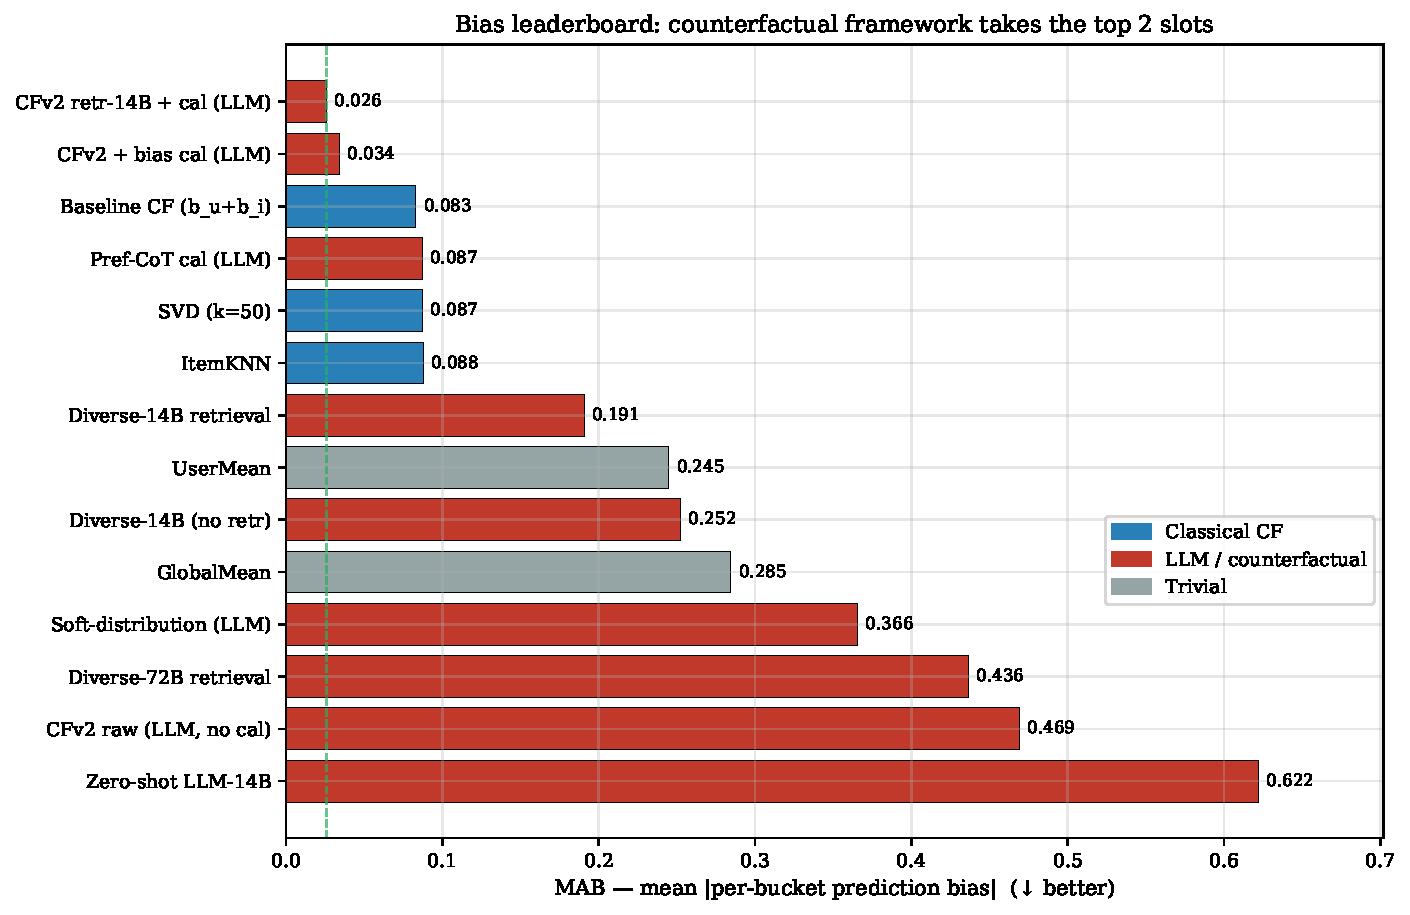
\includegraphics[width=0.95\linewidth]{figures/bias_leaderboard.pdf}

  \vspace{0.3em}
  \footnotesize
  \good{The two counterfactual variants occupy the top two slots} —
  $\mathbf{3\!\times}$ lower MAB than Baseline CF, SVD, or ItemKNN; $\mathbf{24\!\times}$ lower than the zero-shot LLM.
\end{frame}

% =================================================================
\begin{frame}{Ranking Leaderboard: HR@k and NDCG@k}
  \begin{columns}[T,onlytextwidth]
    \begin{column}{0.50\textwidth}
      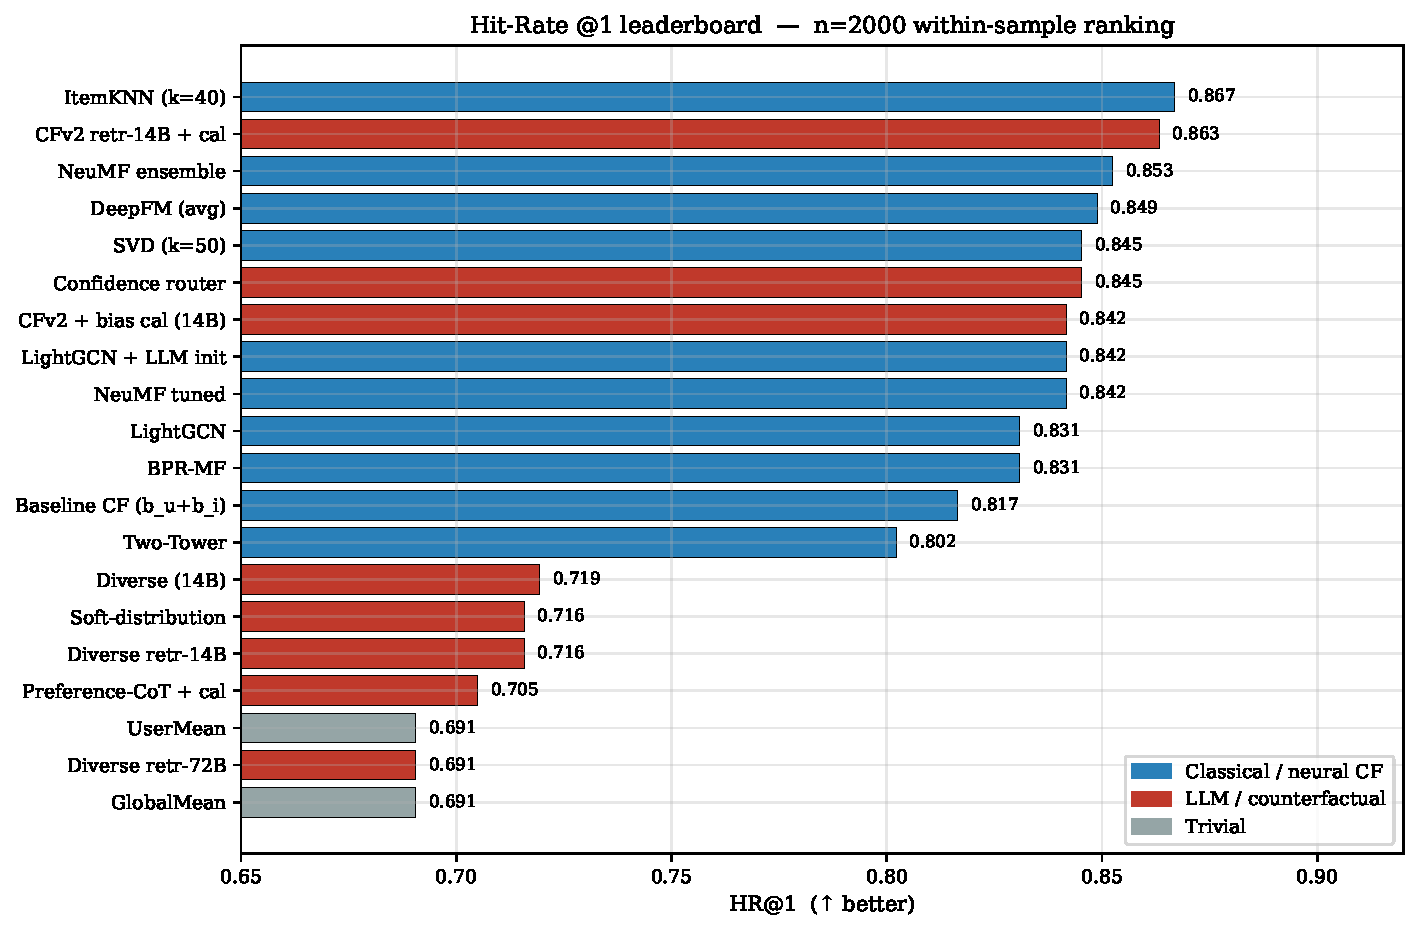
\includegraphics[width=\linewidth]{figures/hr_leaderboard.pdf}
      \begin{center}\scriptsize HR@1 across all methods\end{center}
    \end{column}
    \begin{column}{0.50\textwidth}
      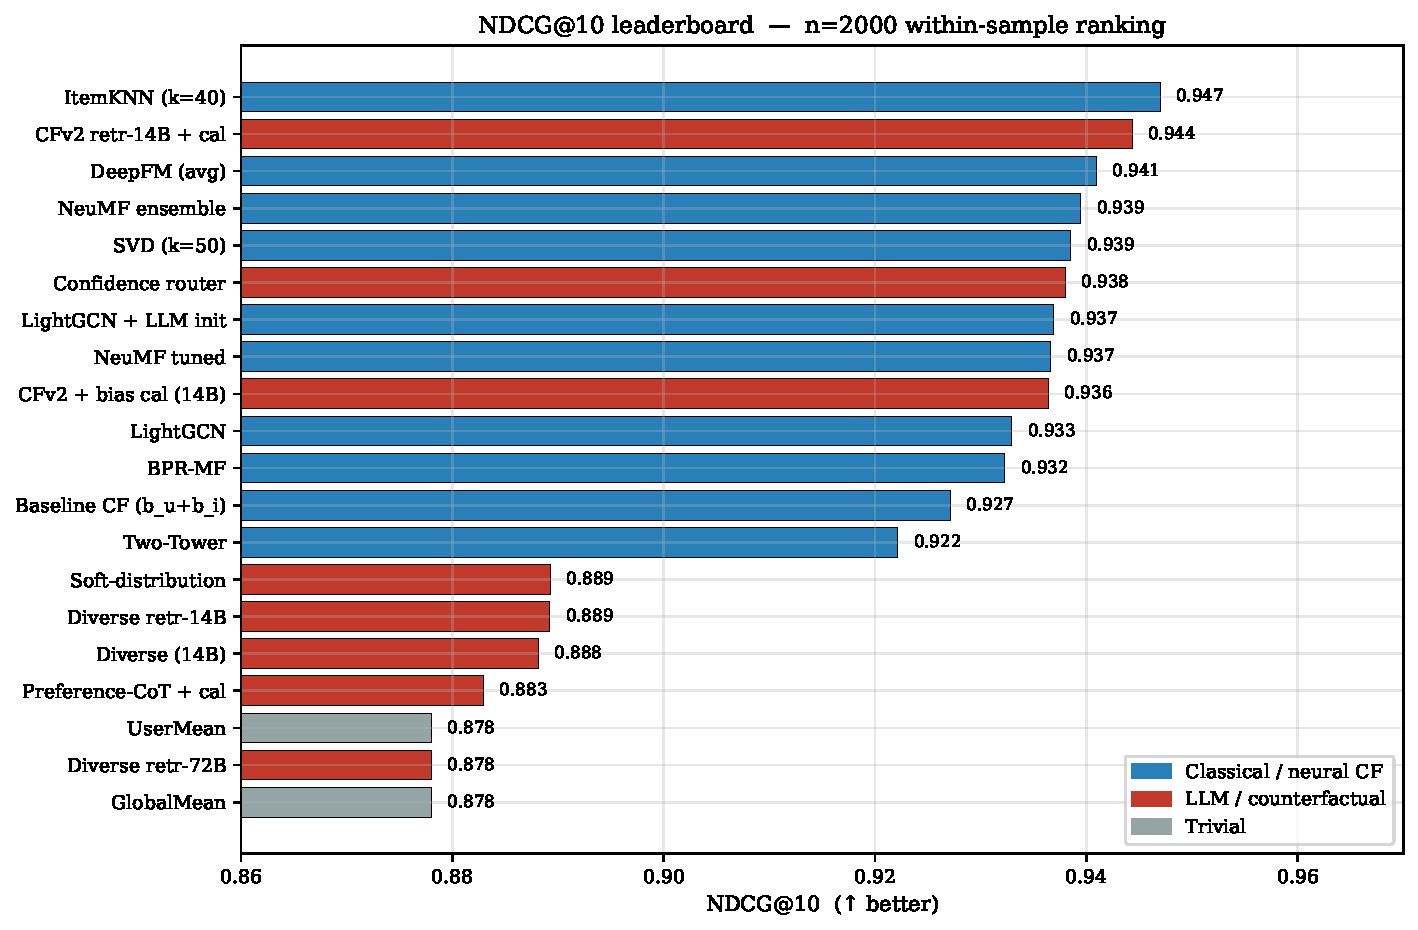
\includegraphics[width=\linewidth]{figures/ndcg_leaderboard.pdf}
      \begin{center}\scriptsize NDCG@10 across all methods\end{center}
    \end{column}
  \end{columns}
  \vspace{0.2em}
  \footnotesize
  Binarisation threshold: rating $\geq 4$ = positive. $n{=}2000$ stratified
  sample, $278$ eligible users, $1{,}045$ positives.\\
  \good{CFv2 retr-14B + cal (our LLM method) ranks 2nd on every metric}
  — HR@1 $=0.863$, NDCG@10 $=0.944$, within $0.3\%$ of ItemKNN's top score.
  Un-anchored LLMs sit at the bottom (HR@1 $\approx 0.70$) — anchoring is
  the key design choice for ranking too.
\end{frame}

% =================================================================
\begin{frame}{Mechanism: Where the Bias Goes}
  \begin{columns}[T,onlytextwidth]
    \begin{column}{0.50\textwidth}
      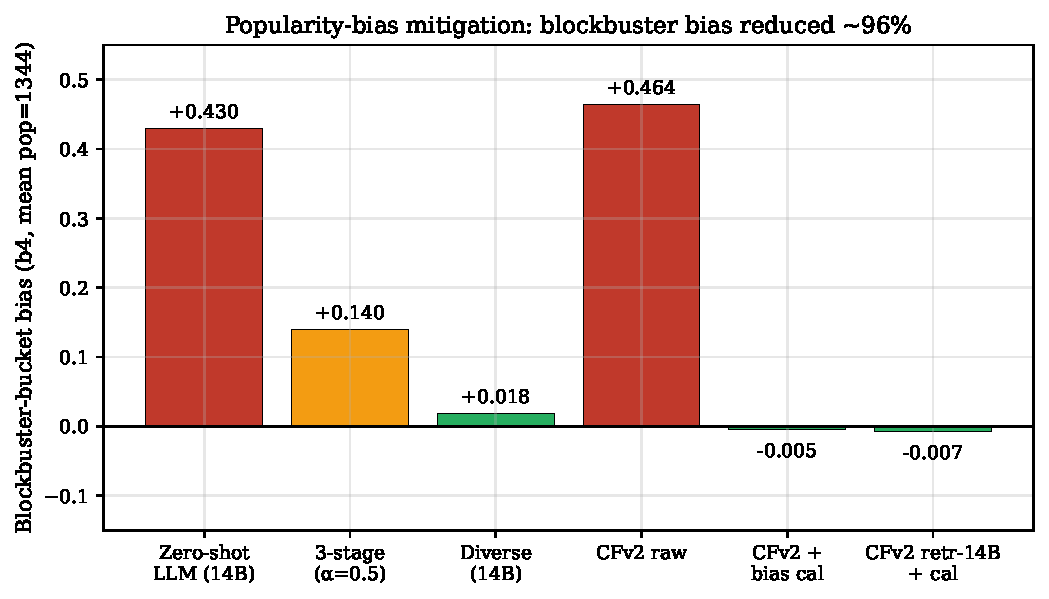
\includegraphics[width=\linewidth]{figures/blockbuster_bias_reduction.pdf}
      \begin{center}\scriptsize
        Blockbuster-bucket bias across stages
      \end{center}
    \end{column}
    \begin{column}{0.50\textwidth}
      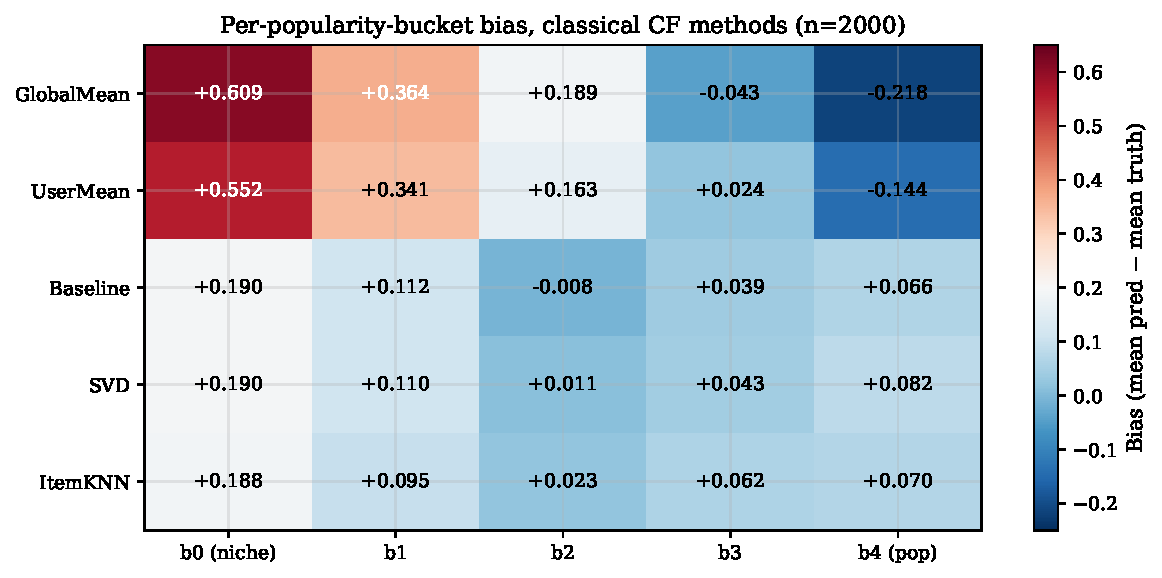
\includegraphics[width=\linewidth]{figures/heatmap_bias_per_bucket.pdf}
      \begin{center}\scriptsize
        Per-bucket bias across classical CF
      \end{center}
    \end{column}
  \end{columns}
  \vspace{0.3em}
  \begin{itemize}\itemsep0pt
    \item \good{Blockbuster bias:} $+0.43$ \ $\to$ \ $-0.018$ \ ($\sim$\textbf{96\% reduction})
    \item \good{MAB:} $0.62$ \ $\to$ \ $0.026$ \ ($\sim$\textbf{96\% reduction})
    \item Every bucket drops to near-zero simultaneously — this is the \emph{causal}
          intervention working, not a constant shift.
  \end{itemize}
\end{frame}

% =================================================================
\begin{frame}{Mechanism in Human Terms: Concrete Case Studies}
  \small
  \begin{columns}[T,onlytextwidth]
    \begin{column}{0.49\textwidth}
      \textbf{\good{Where CF pipeline helped}}\\[0.2em]
      \footnotesize
      \textbf{User 2105, \emph{Star Trek: The Motion Picture} (pop=626), true=2}
      \begin{itemize}\itemsep0pt
        \item \bad{Zero-shot:} ``Likes sci-fi (Jaws, Star Wars, Terminator) $\to$ 5''
        \item \good{Counterfactual:} ``Rated slow-paced films low (Dead Calm, The Edge); Star Trek~I criticised for slow pacing $\to$ 2''
      \end{itemize}
      \vspace{0.4em}
      \textbf{User 1605, \emph{Police Academy 3} (pop=142), true=2}
      \begin{itemize}\itemsep0pt
        \item \bad{Zero-shot:} ``Likes comedies (Princess Bride) $\to$ 4''
        \item \good{Counterfactual:} ``Prefers \emph{sophisticated} comedies (Sound of Music); Police Academy 3 is lowbrow $\to$ 2''
      \end{itemize}
    \end{column}
    \begin{column}{0.49\textwidth}
      \textbf{\bad{Where it hurt (why CFv2 bounds the delta)}}\\[0.2em]
      \footnotesize
      \textbf{User 4352, \emph{Billy Madison} (pop=264), true=5}
      \begin{itemize}\itemsep0pt
        \item \good{Zero-shot:} ``Likes 1990s comedies $\to$ 5'' \,(correct)
        \item \bad{Counterfactual:} ``Sometimes rates musicals low $\to$ 3'' \,(over-corrects)
      \end{itemize}
      \vspace{0.6em}
      \textbf{Lesson.}
      \begin{itemize}\itemsep0pt
        \item 3-stage pipeline \emph{does} select debiased hypotheses (pop-reliance $1.85/10$, plausibility $8.6/10$)
        \item But LLM can over-commit when baseline is already right.
        \item \cf{CFv2's bounded $\Delta\in\{-1,\pm\tfrac12,0,\tfrac12,1\}$} limits drift from a strong CF anchor.
      \end{itemize}
    \end{column}
  \end{columns}
\end{frame}

% =================================================================
\begin{frame}{Does Debiasing Cost Accuracy or Ranking? No.}
  \begin{columns}[T,onlytextwidth]
    \begin{column}{0.55\textwidth}
      \textbf{CFv2 retr-14B + cal vs ItemKNN}
      \begin{itemize}\itemsep0pt
        \item RMSE \good{$0.903$} vs $0.901$ (within $0.3\%$)
        \item HR@1 \good{$0.863$} vs $0.867$ (within $0.5\%$)
        \item NDCG@10 \good{$0.944$} vs $0.947$ (within $0.3\%$)
        \item MAB \good{$0.026$} vs $0.088$ (\textbf{3$\times$ better})
      \end{itemize}
      \vspace{0.3em}
      \textbf{Stacker}
      \begin{itemize}\itemsep0pt
        \item Ridge blend (CF + counterfactual LLM) reaches \good{RMSE $0.876$}.
        \item Closes \textbf{76\%} of the gap to the per-pair oracle ($0.860$).
      \end{itemize}
      \vspace{0.5em}
      \textbf{Stacker v4 composition}
      \begin{itemize}\itemsep0pt
        \item 47\% LLM-derived coefficient mass
        \item 43\% classical/neural CF
        \item 12\% derived meta (genre affinity, log-pop)
      \end{itemize}
    \end{column}
    \begin{column}{0.43\textwidth}
      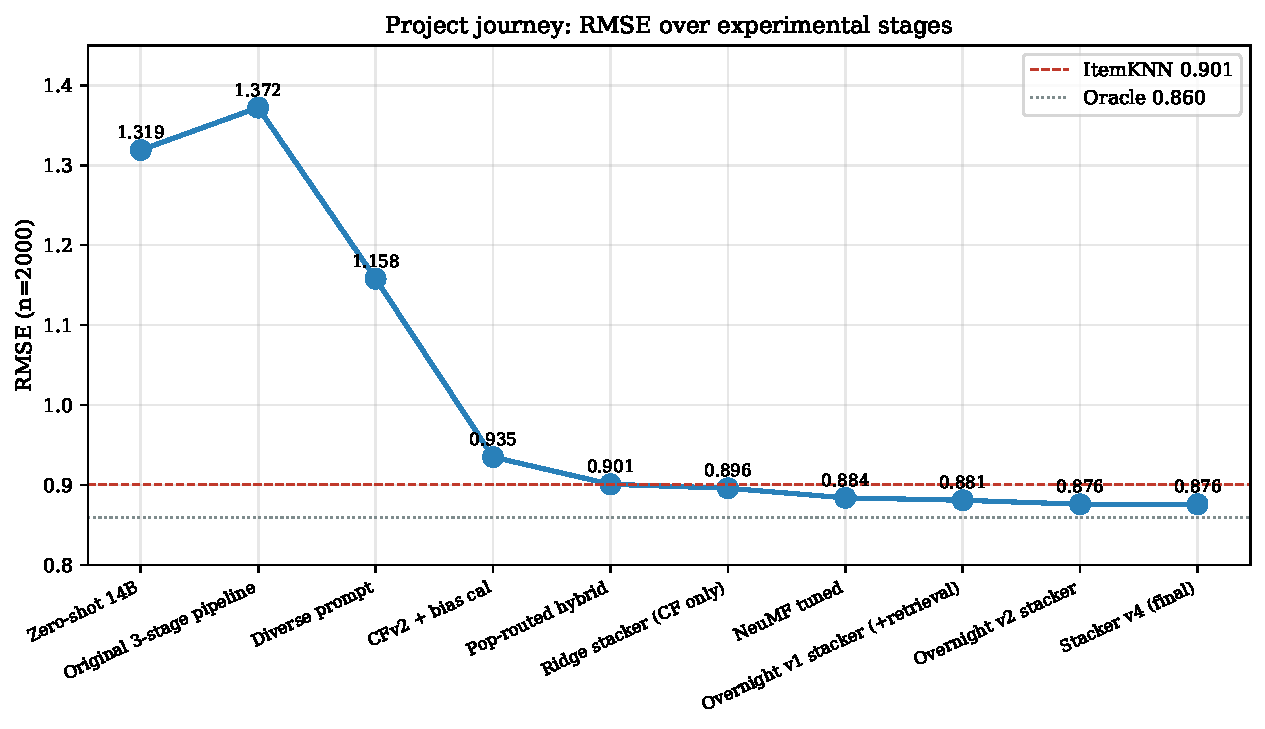
\includegraphics[width=\linewidth]{figures/journey.pdf}
      \begin{center}\scriptsize
        RMSE journey across the project
      \end{center}
    \end{column}
  \end{columns}
\end{frame}

% =================================================================
\begin{frame}{Stacker Inspection: LLM Features Are Not Decoration}
  \begin{columns}[T,onlytextwidth]
    \begin{column}{0.55\textwidth}
      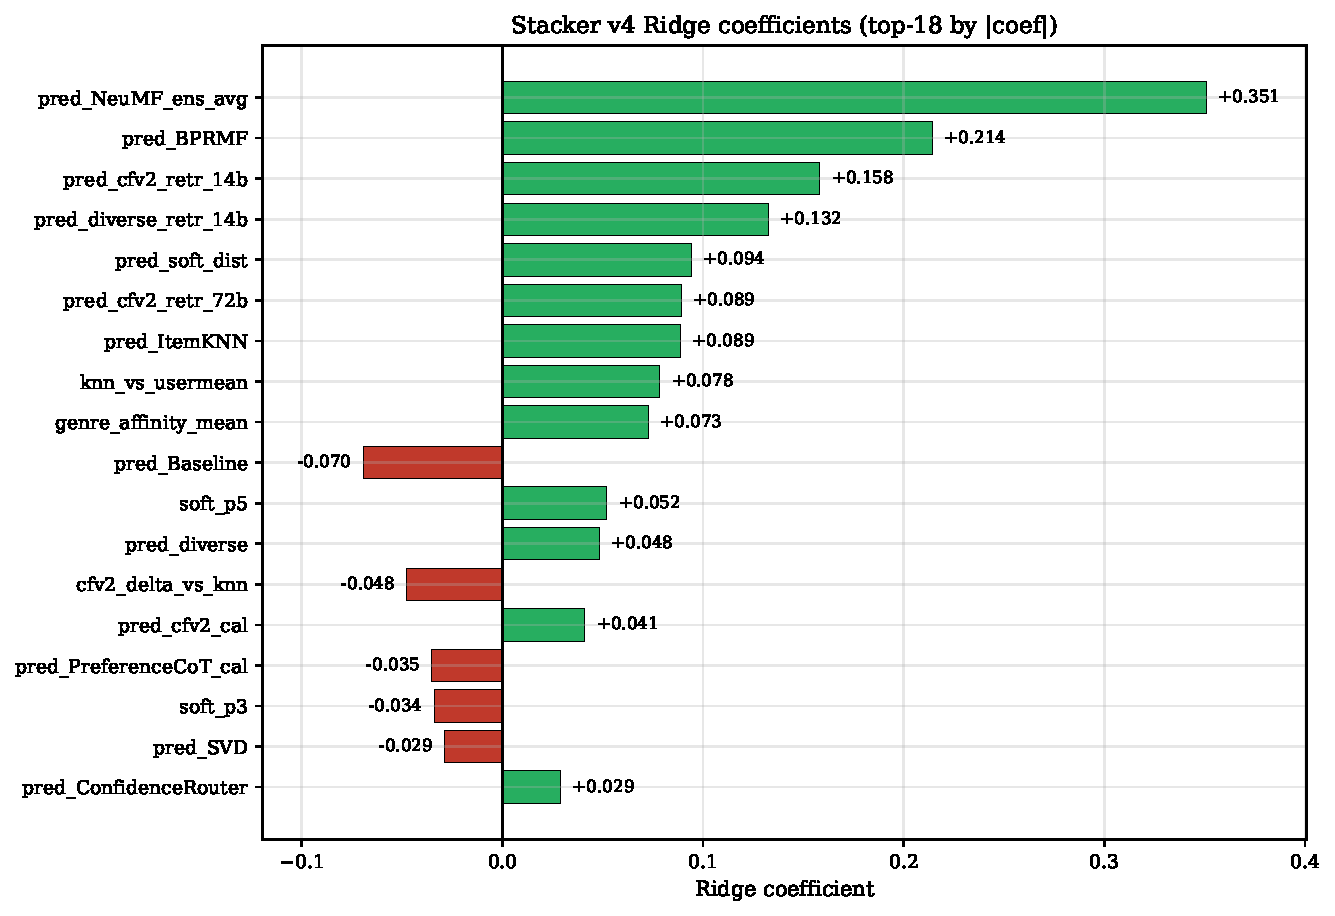
\includegraphics[width=\linewidth]{figures/stacker_coefs.pdf}
    \end{column}
    \begin{column}{0.43\textwidth}
      \textbf{Coefficient-mass accounting}
      \begin{itemize}\itemsep1pt
        \item \good{LLM direct (14 feats)} — $44\%$
        \item \cf{LLM indirect} (embeddings, delta, 3 feats) — $3\%$
        \item \cf{Classical / neural CF (8 feats)} — $43\%$
        \item Derived meta (8 feats) — $12\%$
      \end{itemize}
      \textbf{Top features}
      \begin{itemize}\itemsep0pt\footnotesize
        \item $+0.35$ NeuMF ensemble (CF)
        \item $+0.21$ BPR-MF (CF)
        \item \good{$+0.16$ CFv2 retr-14B (LLM)}
        \item \good{$+0.13$ Diverse retr-14B (LLM)}
        \item \good{$+0.09$ Soft-dist (LLM)}
        \item \good{$+0.09$ ItemKNN (CF)}
      \end{itemize}
      \footnotesize
      4 of the next 6 largest weights are LLM-derived —\\
      remove LLM entirely and RMSE rises from $0.876 \to 0.878$.
    \end{column}
  \end{columns}
\end{frame}

% =================================================================
\begin{frame}{What Didn't Work (and What That Tells Us)}
  \begin{columns}[T,onlytextwidth]
    \begin{column}{0.52\textwidth}
      \textbf{Negative findings}
      \begin{itemize}\itemsep1pt
        \item \bad{TIPS time-awareness is null} on ML-1M's 3-year span — popularity geography too stable.
        \item \bad{3-stage scaffolding isn't the debiaser} — bounded-delta + calibration are.
        \item \bad{Un-anchored LLM prompting} (soft-dist, pref-CoT, logprob) all \emph{increase} bias.
        \item \bad{Confidence router} (LLM meta-learner) is worse than fixed Ridge blend.
        \item \bad{Residual NeuMF, DeepFM, tree stackers}: all overfit.
      \end{itemize}
    \end{column}
    \begin{column}{0.46\textwidth}
      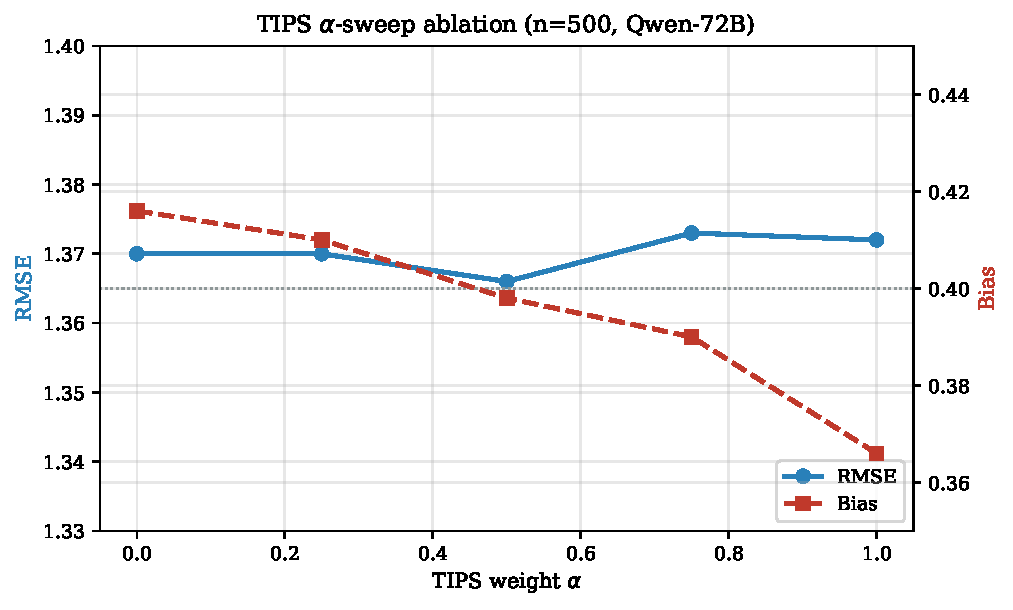
\includegraphics[width=\linewidth]{figures/tips_ablation.pdf}
      \begin{center}\scriptsize
        TIPS $\alpha$-sweep: RMSE flat across all $\alpha$
      \end{center}
    \end{column}
  \end{columns}
\end{frame}

% =================================================================
\begin{frame}{Cold-Start: The Regime Where Pure LLM Wins}
  \begin{columns}[T,onlytextwidth]
    \begin{column}{0.45\textwidth}
      \textbf{On items with pop $=0$ ($n{=}54$)}
      \begin{itemize}\itemsep1pt
        \item ItemKNN collapses to user-bias baseline.
        \item Pure LLM has \good{best MAE} ($0.722$).
        \item A 50/50 LLM+ItemKNN hybrid has \good{best RMSE} ($0.942$).
        \item \textbf{Only regime} where the LLM's external world-knowledge buys RMSE parity.
      \end{itemize}
    \end{column}
    \begin{column}{0.54\textwidth}
      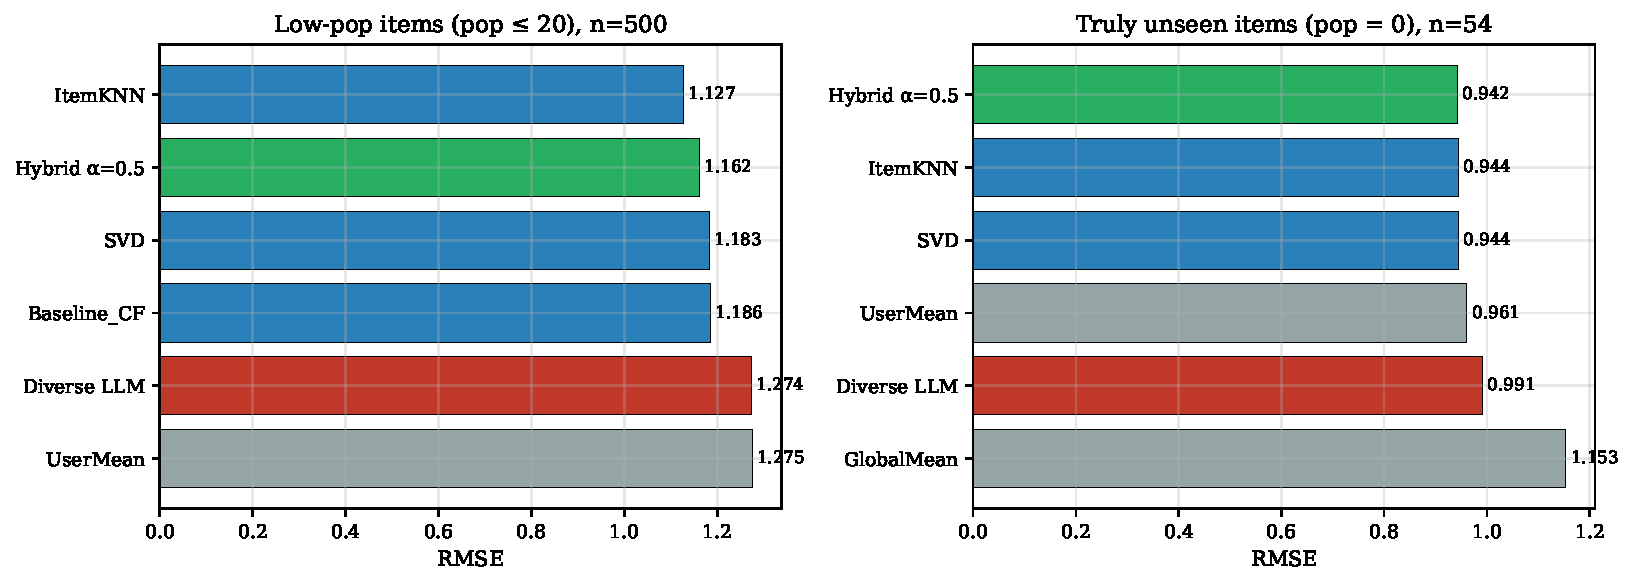
\includegraphics[width=\linewidth]{figures/coldstart.pdf}
    \end{column}
  \end{columns}
\end{frame}

% =================================================================
\begin{frame}{Conclusion \& Recommendation}
  \textbf{Research question.}
  Can counterfactual reasoning mitigate popularity bias in LLM-based rating prediction? \textbf{\good{Yes.}}
  \vspace{0.5em}

  \begin{columns}[T,onlytextwidth]
    \begin{column}{0.52\textwidth}
      \textbf{Primary (bias) outcome}
      \begin{itemize}\itemsep0pt
        \item MAB $0.62 \to 0.026$ \ (\good{96\%} cut)
        \item Blockbuster bias $+0.43 \to -0.018$ \ (\good{96\%} cut)
        \item Top 3 slots on the bias leaderboard
      \end{itemize}
      \textbf{Secondary (accuracy) outcome}
      \begin{itemize}\itemsep0pt
        \item CFv2 retr-14B + cal: RMSE $0.903$
        \item Full Ridge stacker: \good{RMSE $0.876$} (76\% of oracle gap closed)
      \end{itemize}
    \end{column}
    \begin{column}{0.46\textwidth}
      \textbf{Deployment recipe}
      \begin{enumerate}\itemsep0pt
        \item Train ItemKNN (cheap, strong anchor).
        \item Use LLM to emit bounded counterfactual delta; retrieval-augment the prompt.
        \item Apply bias calibration on a held-out slice.
        \item (Optional) Ridge-stack with NeuMF / BPR-MF for further RMSE.
      \end{enumerate}
      \textbf{Future work}
      \begin{itemize}\itemsep0pt
        \item Cross-dataset transfer (ML-100K, Amazon, BookCrossing).
        \item Reasoning-tuned LLMs.
        \item Ranking-level bias (ARP, coverage).
      \end{itemize}
    \end{column}
  \end{columns}
\end{frame}

% =================================================================
\begin{frame}[standout]
  Thank you \\[1em]
  \small Questions? \\[0.3em]
  \textit{Full report, code, and LLM-cache: deterministic seed = 0}
\end{frame}

\end{document}
